\documentclass[letter]{article}
\usepackage{amsmath}
\usepackage{amsfonts}
\usepackage{amssymb}
\usepackage{bm}
\usepackage{ifthen}
\usepackage{fancyhdr}
\usepackage{graphicx}
\usepackage[hidelinks]{hyperref}
\usepackage{xcolor}
\hypersetup{
    colorlinks,
    linkcolor={red!50!black},
    citecolor={blue!50!black},
    urlcolor={blue!80!black}
}

\definecolor{deepblue}{rgb}{0,0,0.5}
\definecolor{deepred}{rgb}{0.6,0,0}
\definecolor{deepgreen}{rgb}{0,0.5,0}

\usepackage{listings}
\usepackage{tkz-graph}
\usetikzlibrary{arrows}
\usepackage{parskip}

% Default fixed font does not support bold face
\DeclareFixedFont{\ttb}{T1}{txtt}{bx}{n}{12} % for bold
\DeclareFixedFont{\ttm}{T1}{txtt}{m}{n}{12}  % for normal

% Python style for highlighting
\newcommand\pythonstyle{\lstset{
language=Python,
basicstyle=\ttm,
otherkeywords={self},             % Add keywords here
keywordstyle=\ttb\color{deepblue},
emph={MyClass,__init__},          % Custom highlighting
emphstyle=\ttb\color{deepred},    % Custom highlighting style
stringstyle=\color{deepgreen},
frame=tb,                         % Any extra options here
showstringspaces=false            % 
}}


% Python environment
\lstnewenvironment{python}[1][]
{
\pythonstyle
\lstset{#1}
}
{}

% Python for external files
\newcommand\pythonexternal[2][]{{
\pythonstyle
\lstinputlisting[#1]{#2}}}

% Python for inline
\newcommand\pythoninline[1]{{\pythonstyle\lstinline!#1!}}


%%%
% Set up the margins to use a fairly large area of the page
%%%
\oddsidemargin=.2in
\evensidemargin=.2in
\textwidth=6in
\topmargin=-.5in
\textheight=9in
\parskip=.07in
\parindent=0in
\pagestyle{fancy}



%%%
% Set up the header
%%%
\newcommand{\setheader}[6]{
	\lhead{{\sc #1}\\{\sc #2} ({\small \it \today})}
	\rhead{
		{\bf #3} 
		\ifthenelse{\equal{#4}{}}{}{(#4)}\\
		{\bf #5} 
		\ifthenelse{\equal{#6}{}}{}{(#6)}%
	}
}

\makeatletter
\newcommand{\escapeus}{\begingroup\@makeother\_\@escapeus}
\newcommand*{\@escapeus}[1]{#1\endgroup}
\makeatother

%%%
% Set up some shortcut commands
%%%
\newcommand{\R}{\mathbb{R}}
\newcommand{\N}{\mathbb{N}}
\newcommand{\Z}{\mathbb{Z}}
\newcommand{\C}{\mathbb{C}}
\newcommand{\Proj}{\mathrm{proj}}
\newcommand{\Perp}{\mathrm{perp}}
\newcommand{\proj}{\mathrm{proj}}
\newcommand{\Span}{\mathrm{span}}
\newcommand{\Null}{\mathrm{null}}
\newcommand{\Rank}{\mathrm{rank}}
\newcommand{\mat}[1]{\begin{bmatrix}#1\end{bmatrix}}
\newcommand{\var}[1]{{$\langle$\it #1$\rangle$}}
\newcommand{\Code}[1]{\texttt{\escapeus #1}}
\DeclareMathOperator{\Tr}{Tr}

%%%
% This is where the body of the document goes
%%%
\begin{document}
	\setheader{MAT335}{Homework 4 }{Due: 11:59pm April 6}{}{}{}

	\begin{enumerate}
		\item For a dynamical system $(T,X)$, a point $x\in X$ is called \emph{eventually periodic} if there 
			exists $m>m'$ so that $T^mx=T^{m'}x$.
		\begin{enumerate}
			\item Let $(T,[0,1))$ be the doubling map and let $(\sigma,\Omega)$ be the full two shift.
				For each system, give an example of (i) a point that is eventually periodic, and (ii)
				a point that is eventually periodic but \emph{not} periodic.
				
				\begin{quote}
				    Recall, the doubling map is defined by, 
				    \[
				        T: [0,1) \to [0,1); x \mapsto 2x \ mod \ 1.
				    \]
				    A periodic point can be given by $\frac{1}{5}$ and an eventually periodic point that is not periodic is given by $\frac{11}{24}$:
                    \[
                        \frac {11}{24} \mapsto \frac{11}{12} \mapsto 
                        \frac {5}{6} \mapsto {\frac {2}{3}} \mapsto 
                        {\frac {1}{3}} \mapsto {\frac {2}{3}}\mapsto 
                        {\frac {1}{3}} \mapsto \cdots
                    \]
                    
                    Recall, the full two shift, $(\sigma, \Omega)$, is defined as,
                        $\Omega=\{0,1\}^\N$ and  $\sigma:\Omega\to\Omega$,
                        \[
                        	\sigma(a_0,a_1,a_2\ldots) = (a_1,a_2,a_3\ldots).
                        \]
                    Then, a periodic point can be given by the base 2 expansion of $\frac{1}{5} = 0.0011001100110011..._2 $. An eventually periodic point that is not periodic is given by the base 2 expansion of the point $\frac{11}{12} = 0.01110101010101..._2$.
                    \[
                      \sigma^i(p) = \sigma^{i+2}(p), \forall i > 5  
                    \]
                    That is, after shifting 5 times or more, $\frac{11}{12}$ has period of 2.
				\end{quote}
			\item Let $\C$ be the coding function for the doubling map with the usual partition ($\mathcal P_0=[0,1/2)$
				and $\mathcal P_1=[1/2,1)$).

				Prove $\C(x)$ is eventually periodic in $(\sigma, \Omega)$ if and only if $x$ is eventually
				periodic in $(T,[0,1))$.
			\begin{quote}
			    
			 %   We can visualize this encoding with a circle map that wraps the number line from 0 to 1 into a circle. Then, the partitions are the two halves to the circle map. 
			    
			 %   We know the transformation of $(\sigma, \Omega)$ will shift a string made from a binary alphabet one element to the right.
			    
			 %   Next, we can form a bijection between the encoded doubling map to a binary expansion of x. This is because [TODO]. We also know that shifting a binary string to the left corresponds to multiplication by 2 which is what the doubling transformation is doing.
			    
			 %   Thus, we see that if a value in $\C(x)$ is eventually periodic in $(\sigma, \Omega)$ if and only if $x$ is eventually periodic in $(T,[0,1))$.
			 
			 Any $x \in [0, 1]$ has a binary expansion given by $\displaystyle x = \sum_{n=0}^{\infty} \frac{x_n}{2^{n+1}}$ for $x_n \in \{0,1\}$. 
			 
 		     For $\C(x)$, we may choose the encoding to be the binary values $0$ and $1$. Then for the doubling map with the defined partitions, $\C(x)$ will encode values $x_n$ to 0 if $T^n x \in \mathcal P_0$ otherwise it will encode $x_n$ to 1. So $\C: [0,1) \mapsto \Omega$
			 
			Next, we can define $\pi: \Omega \mapsto [0,1)$ by 
			\begin{align*}
			     \pi(x_0, x_1, x_2, \cdots) 
			     &= \sum_{n=0}^{\infty} \frac{x_n}{2^{n+1}} 
			     \intertext{Then,}
			     T(\pi(x_0, x_1, x_2, \cdots)) 
			     &= T \Big (  \sum_{n=0}^{\infty} \frac{x_n}{2^{n+1}} \Big )\\
			     &= x_0  +\sum_{n=1}^{\infty} \frac{x_n}{2^{n}} \ mod \ 1\\
			     &= \sum_{n=1}^{\infty} \frac{x_n}{2^n}.
			     \intertext{Since $x_0 = 0$}
			     \intertext{Alternatively, }
			     \pi(\sigma(x_0, x_1,  x_2, \cdots ))
			     &= \pi(x_1, x_2, \cdots)\\
			     &= \sum_{n=1}^{\infty} \frac{x_n}{2^n}.
			\end{align*}
			Thus, $T \circ \pi = \pi \circ \sigma$. We see that $\pi$ is surjective and is injective on the set  $[0, 1)$ after removing binary expansions ending in all 0s or 1s (dyadic rationals). This is because these rationals all have two binary representations so are not unique.
			
			Since it is trivial to see that dyadic rationals will have period of length 1 in both systems, we may remove them and only consider the remaining values in $[0,1)$ for which there is a bijection. Since both mappings will have the same binary representation, it is clear that $\C(x)$ is eventually periodic in $(\sigma, \Omega)$ if and only if $x$ is eventually periodic in $(T,[0,1))$
			\end{quote}
			
			
			\item Prove that $\C(x)$ is eventually periodic if and only if $x$ is a rational number.

			\begin{quote}
		        As we have already shown that $\C(x)$ is surjective with the base 2 expansion of a number $x \in [0,1)$, we know that $\C(x)$ will always correspond to a binary representation of a number in $[0,1)$. We only need to prove that the binary expansion of any rational number is periodic.
		        
		        We see that if $x = \frac{1}{n}$ for $n>0$ we have $2^m \equiv 1 \mod n$. Then for some $a, 1 \leq a < 2^m-1$ we have,
		        \begin{align*}
		            \dfrac{1}{n} &= \dfrac{a}{2^k-1} \\
		            &= \dfrac{a}{2^k} + \dfrac{a}{2^{2k}} + \dfrac{a}{2^{3k}} + \cdots
		        \end{align*}
		        This is equal to the number $x  \in [0,1) $ with base 2 expansion of $0.\overline{00\dots01}$ where there are $k-1$ $0$s. Thus we see that any rational number will have a periodic binary expansion.
			\end{quote}

			\item Prove that a binary expansion of a number in $[0,1)$  (viewed as an element of $(\sigma, \Omega)$ 
				is eventually periodic if and only
				if that number is rational. (\emph{Hint: $\C(x)$ is always a binary expansion, but not all
				binary expansions come from codings}).
				
			\begin{quote}
			    The previous proofs have already shown that all binary expansions $\mathcal C = \{ \C(x) | x \in [0,1) \}$ will have a periodic expansion iff $x$ is rational. We can see that $\mathcal B = \Omega - \mathcal C$ will be the set of possible binary expansions that do not come from the set of all possible codings.
			    
			    We find that elements of $\mathcal B$ must be irrational because they cannot be represented in the following form which previously represented any periodic base-2 expansion,
		        \begin{align*}
		            \dfrac{1}{n} &= \dfrac{a}{2^k-1} 
		            = \dfrac{a}{2^k} + \dfrac{a}{2^{2k}} + \dfrac{a}{2^{3k}} + \cdots
		        \end{align*}
			\end{quote}
				
			\item Prove that the base $n$ expansion of a number in $[0,1)$ is eventually periodic if an only if that
				number is rational.
			\begin{quote}
			    We can use the following identity,
			    \begin{align*}
			        \sum_{n=1}^\infty p^{-kn}
			        &= \frac{p^{-k}}{1-p^{-k}}
			        =\frac{1}{p^k-1}\\
			        &= 
			    \end{align*}
			    This is equal to the number $x \in [0,1)$ with base $p$ expansion of $0.\overline{00\dots01}$ where there are $k-1$ $0$s. Thus any base p expansion of a number in $[0,1)$ is eventually periodic iff that number is rational
			\end{quote}
		\end{enumerate}

        \newpage
		\item Let $(\sigma, \Omega)$ be the full two-shift. Let $G\subseteq\Omega$ 
			bet the set of sequences without two ones in a row.
			Let $X\subseteq \Omega$ be the set of sequences without \emph{three} ones in a row.
			\begin{enumerate}
				\item Show that $(\sigma, X)$ is a subshift.
			    \begin{quote}
			        We know that $X$ is $\sigma$-invariant, that is $\sigma(X) = X$. This is because after shifting any sequence without three ones in row, the resulting sequence will also not contain three ones in a row.
			        
			        We also know that $X$ is a closed set because it contains all its limit points. This is true because infinite applications of sigma can not produce sequences containing three consecutive ones in a row if the original sequence did not contain three consecutive ones.
			        
			        Thus, $(\sigma, X)$ is a subshift.
			    \end{quote}

				\item A \emph{two-step} Markov chain is a Markov chain where the transition probabilities
					between states depend on the current state \emph{and} the previous state. 
					
					A \emph{two-step} Markov chain on a state space $S$ can be thought of as a 
					one-step (regular) Markov chain on the state space $S\times S$. For example, let
					$\mathcal M$ be the Markov
					chain on states $0$ and $1$ with equal transition probabilities.
					Normally, $\mathcal M$ has a graph like this:

					\begin{center}
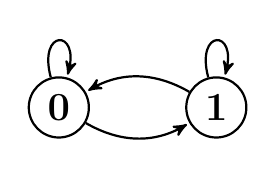
\begin{tikzpicture}[->,>=stealth',shorten >=1pt,auto,node distance=2cm,
                thick,main node/.style={circle,draw,font=\Large\bfseries}]
  \node[main node] (1) {0};
  \node[main node] (2) [right of=1] {1};


  \path
    (2) edge [loop above] (2);

  \path
    (1) edge [loop above] (1)
	edge [bend right] (2)
    (2) edge [bend right] (1)
    ; 
\end{tikzpicture} 
			\end{center}
		However, we can also model $\mathcal M$ as a Markov chain $\mathcal M'$
		with state space $00$, $01$, $10$, and $11$ and transition graph like this:
		\begin{center}
            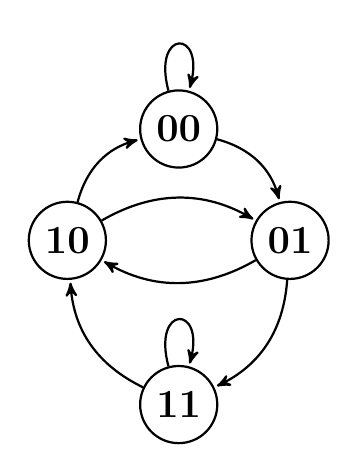
\begin{tikzpicture}[->,>=stealth',shorten >=1pt,auto,node distance=2cm, thick,main node/.style={circle,draw,font=\Large\bfseries}]
              \node[main node] (00) {00};
              \node[main node, yshift=-1.5cm] (11) [below of=00] {11};
              \node[main node] (01) [below right of=00] {01};
              \node[main node] (10) [below left of=00] {10};
            
            
              \path
                (11) edge [loop above] (11);
            
              \path
                (00) edge [loop above] (00);
            
              \path
                (11) edge [bend left] (10)
                (01) edge [bend left] (10)
                (01) edge [bend left] (11)
                (10) edge [bend left] (00)
                (10) edge [bend left] (01)
                (00) edge [bend left] (01)
                ; 
            \end{tikzpicture} 
    	\end{center}
		Explain how $\mathcal M'$ models $\mathcal M$. In particular, explain why the graph for $\mathcal M'$ has no edge between $00$ and $11$.
        \begin{quote}
            We know the states of $\mathcal M'$ capture the previous and current state of $\mathcal M$. $\mathcal M'$ can be understood as being a model of $\mathcal M$ if we consider $00 \equiv 0$, $11 \equiv 1$ and suppose the additional transitions for the states $01$ and $10$ have equivalent steady state probabilities for $0 \to 1$, $1 \to 0$ and self transitions $0 \to 0$, $1 \to 1$ respectively. Moreover, the additional states add extra information about the transition probabilities given the previous state.
            
            There is no edge between $00$ and $11$ because it is not possible for a state $0$ to transition to state $1$ without having a previous state of $0$.
        \end{quote}
    
		\item Let $\mathcal M_G$ be a Markov chain whose set of realizations is $G$.
			\begin{enumerate}
				\item Draw a graph for $\mathcal M_G$ and find its associated transition matrix.
    		    \begin{equation*}
                    \begin{aligned}[c]
                        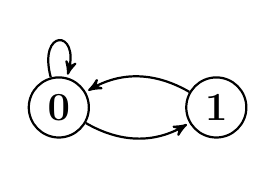
\begin{tikzpicture}[->,>=stealth',shorten >=1pt,auto,node distance=2cm,
                        thick,main node/.style={circle,draw,font=\Large\bfseries}]
                        \node[main node] (1) {0};
                        \node[main node] (2) [right of=1] {1};
                        
                        \path
                        (1) edge [loop above] (1)
                        edge [bend right] (2)
                        (2) edge [bend right] (1)
                        ; 
                        \end{tikzpicture} 
                    \end{aligned}
                    \ \ \ \ \
                    \begin{aligned}[c]
                        \mathcal M_G  
                        =
                        \mat{
                            0.5& 1 \\
                            0.5& 0 \\
                        }
                        =
                        \mat{
                            1& 1 \\
                            1& 0 \\
                        }
                    \end{aligned}
                \end{equation*}
			
				\item Use the transition matrix for $\mathcal M_G$ to compute the entropy of $(\sigma, G)$.
				\begin{quote}
				    We may use the fact that for subshifts of finite type, topological entropy coincides with the logarithm of the spectral radius of the transition matrix\footnote{\text{http://www.scholarpedia.org/article/Topological\_entropy\#Topological\_entropy\_in\_some\_special\_cases}}.
				
    				Let $\lambda^*$ be the spectral radius, i.e. the largest eigenvalue modulus of the adjacency matrix. Then we can calculate the topological entropy as,
    				\begin{align*}
    				    \mathcal H(G) &= \lim_{n\to \infty} 
    				    \frac{log(\text{\# words of length n in G})}{log(\text{\# of words of length n in } \Omega)}\\[8pt]
    				    &\equiv log(|\lambda^*|) 
    				    = log \Big ( \Big | \frac{(1+ \sqrt{5}))}{2} \Big | \Big) 
    				    = 0.4812118250...
    				\end{align*}
				\end{quote}

				\item Model $\mathcal M_G$ as a two-step Markov chain  $\mathcal M_G'$, which can be viewed as a Markov chain
					with state space $\{00,01,10,11\}$. 					Draw the graph associated with $\mathcal M_G'$ and find its transition matrix.
                    \begin{equation*}
                    \begin{aligned}[c]
                        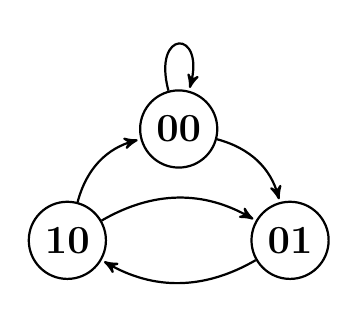
\begin{tikzpicture}[->,>=stealth',shorten >=1pt,auto,node distance=2cm, thick,main node/.style={circle,draw,font=\Large\bfseries}]
                        \node[main node] (00) {00};
                        \node[main node] (01) [below right of=00] {01};
                        \node[main node] (10) [below left of=00] {10};
                        \path
                        (00) edge [loop above] (00);
                        \path
                        (01) edge [bend left] (10)
                        (10) edge [bend left] (00)
                        (10) edge [bend left] (01)
                        (00) edge [bend left] (01)
                        ; 
                        \end{tikzpicture} 
                    \end{aligned}
                    \ \ \ \ \
                    \begin{aligned}[c]
                        \mathcal M_G  
                        =
                        \mat{
                            0.5& 0& 0.5 \\
                            0.5& 0& 0.5 \\
                            0& 1& 0 
                        }
                        =
                        \mat{
                            1& 0& 1 \\
                            1& 0& 1 \\
                            0& 1& 0 
                        }
                    \end{aligned}
                \end{equation*}
				\item Using the transition matrix for $\mathcal M_G'$, compute the entropy of $(\sigma, G)$.
				\begin{quote}
    				Let $\lambda^*$ be the spectral radius, i.e. the largest eigenvalue of the adjacency matrix. Then we can calculate the topological entropy as
    				\begin{align*}
    				    \mathcal H(G) &= \lim_{n\to \infty} 
    				    \frac{log(\text{\# words of length n in G})}{log(\text{\# of words of length n in } \Omega)}\\[8pt]
    				    &= log(|\lambda^*|) 
    				    = log \Big ( \Big | \frac{(1+ \sqrt{5})}{2} \Big | \Big ) 
    				    = 0.4812118250...
    				\end{align*}
				\end{quote}
			\end{enumerate}
	    
		\item Can $X$ be modeled by a one-step Markov chain? Why or why not?
		\begin{quote}
		    Recall, $X$ is the subset of sequences without 3 consecutive $1$'s. The one-step Markov chain could not model this as removing a transition or edge from 1 to itself would also remove all sequences with two consecutive 1s.
		\end{quote}
		\newpage
		\item Find the entropy of $(\sigma, X)$.
		\begin{quote}
		    We see that $X \subset G$ without any transitions or edges from state $11$ to itself so it can be modeled with the two-state markov chain and its entropy found,
            \begin{equation*}
            \begin{aligned}[c]
                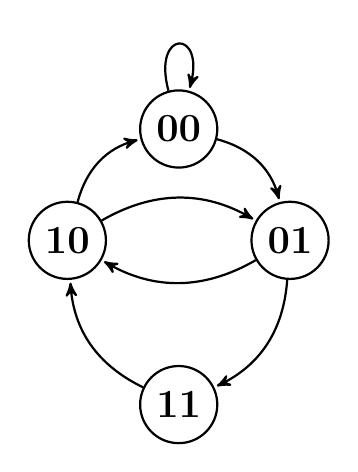
\begin{tikzpicture}[->,>=stealth',shorten >=1pt,auto,node distance=2cm, thick,main node/.style={circle,draw,font=\Large\bfseries}]
                \node[main node] (00) {00};
                \node[main node, yshift=-1.5cm] (11) [below of=00] {11};
                \node[main node] (01) [below right of=00] {01};
                \node[main node] (10) [below left of=00] {10};
                
                \path
                (00) edge [loop above] (00);
                
                \path
                (11) edge [bend left] (10)
                (01) edge [bend left] (10)
                (01) edge [bend left] (11)
                (10) edge [bend left] (00)
                (10) edge [bend left] (01)
                (00) edge [bend left] (01)
                ; 
                \end{tikzpicture}  
            \end{aligned}
            \ \ \ \ \ \
            \begin{aligned}[c]
                \mathcal M_G  
                =
                \mat{
                    1& 0& 1& 0 \\
                    1& 0& 1& 0 \\
                    0& 1& 0& 1 \\
                    0& 1& 0& 0  \\
                }
            \end{aligned}
            \ \ \ \ \ \ 
            \begin{aligned}[c]
                \mathcal H(G)
                &= log(|\lambda^*|) \\
                &= log(1.83929) \\
                &= 0.609380...
            \end{aligned}
        \end{equation*}
		\end{quote}
		
		\end{enumerate}
            
        \newpage
		\item Let $(\sigma, \Omega)$ be the full two shift.
		\begin{enumerate}
			\item Prove that $(\sigma, \Omega)$ is \emph{expansive}.
			\begin{quote}
			    Recall, $(\sigma, \Omega)$ is expansive if for any $x, y \in \Omega$,  if $x \neq y$ then for some $n$ and some $\epsilon > 0$, $d(\sigma^n(x), \sigma^n(y)) > \epsilon $.
			    
			     Suppose $(a_n), (b_n) \in  \Omega $ and $(a_n)\neq(b_n)$, then for some $K \in \N,a_K \neq b_K$. Therefore $d(\sigma^K((a_n)), \sigma^K((b_n))) \geq 1$. So the full two shift is an expansive dynamical system.
			\end{quote}
		
			\item Prove that $(\sigma, \Omega)$ is \emph{transitive}.
			\begin{quote}
                Recall, the point $x \in \Omega$ is called transitive if $ \overline{ \mathcal O (x) } = \Omega$, where $\overline{ \mathcal O(x) }$ the closure of the orbit. The system $(\sigma, \Omega)$ is transitive if there exists a transitive point in $\Omega$. 
                
                We claim that there exists a $y\in \Omega$ such that $\overline{ \mathcal O (y) } = \Omega$.
			    Then, for any $\alpha \in \Omega$, we can choose an arbitrary $\epsilon > 0$, and choose $n$ such that $2^{-n} < \epsilon$. Since $\alpha$ will contain some finite $n$ symbols and since $y$ contains all lists of finite symbols, the contents of $\alpha$ must be in $y$ at some index $j$. Then, by shifting $y$ to this index $j$ will reduce the distance to any arbitrary value, i.e. $d(\sigma^k(y), \alpha) < \epsilon$ for some $k$. We can see that this is the definition for $y$ having a dense orbit, which means that $(\sigma, \Omega)$ is transitive.

                We may choose the base 2 expansion of some transcendental irrational to be $y$, then we know it will be neither periodic nor eventually periodic and will contain all possible sequences of binary values.
			\end{quote}
			
			\item Show that $(\sigma, \Omega)$ is \emph{chaotic}.
    			\begin{quote}
    			    By our definition, the dynamical system $(\sigma, \Omega)$ is chaotic if it is both expansive and transitive. 
    			\end{quote}
			\item Let $(T,X)$ be a dynamical system and let $x,y\in X$. We say $x$ and $y$ are
				\emph{$\delta$-correlated for $n$ steps} if the distance between $T^ix$ and $T^iy$ is
				at most $\delta$ for $i=0,\ldots, n$.

				Let $x,y\in \Omega$ be points that are at distance $2^{-k}$ of each other. For how many steps will
				$x$ and $y$ be $\delta$-correlated when $\delta=1/4$?
				\begin{quote}
				    If $d(x, y) = 2^{-k}$ we know $k = min_k\{j: x_j \neq y_j \}$ is the number of steps x and y will be $\delta$-correlated. We also have that $d(T^{i}x, T^{i}y) \leq \frac{1}{4} = 2^{-2}$. Thus, $x$ and $y$ be $\delta$-correlated for $2$ steps.
				\end{quote}
			\item If $(T,X)$ is a chaotic dynamical system, can two points be $\delta$-correlated indefinitely? What implications
				does this have for measurement error?
			\begin{quote}
			    For two points to be $\delta$-correlated indefinitely means that the distance between $T^nx$ and $T^ny \leq \delta$ for all $n \in \N$. 
			    
			    If $X$ is finite, we may choose some $\delta$ outside the radius of the system $(T,X)$ so that two points will be  $\delta$-correlated indefinitely.
			    
    		    However, if $(T,X)$ is infinite and chaotic or we pick a point within the radius then, because the system is expansive we know there exists $\epsilon>0$, so that if $x,y \in \Omega$ and $d(T^n(x),T^n(y)) \leq \epsilon$ for every $n \in \N$ then, $x=y$. So two points $x \neq y$ will not be $\delta$-correlated indefinitely in an infinite choatic dynamical system or for some choices of $\delta$ inside the bounds of a finite system.
    		    
    		    If you can always pick a small enough $\delta$ so that nothing is delta correlated then you will have a minimum bound on your measurement error. Conversely, if you pick a large enough $\delta$ outside the system, you have a maximum bound on your measurement error.
			    
			 %   If $(T,X)$ is chaotic then it is expansive, meaning $ d(T^n(x),T^n(y)) > \epsilon$ for some $n$ for the systems expansive constant $\epsilon > 0$. Thus it is possible for two points in a chaotic dynamical system to be indefinitely $\delta$-correlated so long as $\delta > \epsilon$. 
			    
			\end{quote}
		\end{enumerate}

    \newpage
	\item Two dynamical systems $(T, X)$ and $(S,Y)$ are called \emph{conjugate} if there exists a continuous, invertible
		function $\Phi:Y\to X$ so that $T=\Phi^{-1}\circ S\circ \Phi$. In this case, $\Phi$ is called a \emph{conjugacy}.

		The systems are called \emph{semi-conjugate} if there
			exist continuous, onto function $\Phi:Y\to X$ so that
			$T\circ\Phi$ = $\Phi\circ S$. In this case, $\Phi$ is called a \emph{semi-conjugacy}.


		\begin{enumerate}
			\item Let $(T,X)$ and $(S,Y)$ be conjugate dynamical systems.
				\begin{enumerate}
					\item Show that if there exists a point of period $k$ in $Y$, there exists a point
						of period $k$ in $X$.
						
					\begin{quote}
					    Since $(T,X)$ and $(S,Y)$ are conjugate, we have,
					    \begin{align*}
					        T &= \Phi^{-1}\circ S\circ \Phi \\
					        T^k &= \Phi^{-1}\circ S^k \circ \Phi \\
					        S^k &= \Phi \circ T \circ \Phi^{-1}
					    \intertext{Then for $y\in Y$,}
					        y &= S^k y \\
					        \implies \Phi^{-1} \circ \Phi y &=  \Phi^{-1} \circ S^k \circ \Phi y \\
					        y &= T^k y.
					        \intertext{Since $\Phi$ is bijective we know there will be a unique $x \in X$,}
					        y &= \Phi^{-1}(x) \\
					        \implies x &= T^k x\\
					       % x &= \Phi \circ T^k \circ\Phi^{-1}x\\
					       % x &= S^k x.
				        \intertext{Therefore if a point in $Y$ has period $k$, a point in $X$ will also have period $k$.}
					    \end{align*}
					\end{quote}
					
					\item Show that if $(S,Y)$ is transitive, then $(T,X)$ is transitive.
					\begin{quote}
					    \vspace*{-5mm}
					    \begin{align*}
					        \intertext{If $(S,Y)$ is transitive, then for some $y \in Y$ we have,}
					        \overline{\mathcal O(y)} &= Y\\
					       &= \bigcap_{n \in \N}  {\{ S^k(y):k>n\}}.\\
					        \intertext{Since $\Phi$ forms a bijection between $Y$ and $X$, for each point in $Y$ from the closure of the orbit of $y$ there will be a unique point in $X$}
					        \overline{\mathcal O(y)} 
					        = \overline{\mathcal O(\Phi^{-1} \circ \Phi (y))} 
					        &= \bigcap_{n \in \N} {\{ \Phi^{-1} \circ S^k \circ \Phi (y):k>n\}}\\
					        &= \bigcap_{n \in \N} {\{ T^k (y):k>n\}}\\
					        &= X
					        \intertext{Thus, if $(S,Y)$ is transitive, then $(T,X)$ is also transitive }
					    \end{align*}
					\end{quote}  
					  
					
					\item Is it true that if $(S,Y)$ is expansive, then $(T,X)$ is necessarily expansive?
				    \begin{quote}
				        \vspace{-8mm}
				        \begin{align*}
				            \intertext{If $X$ and $Y$ are compact, then $\Phi$ is uniformly continuous so there exists an $\alpha > 0$ such that}
				            d(\Phi(y_1)), \Phi(y_2)) \leq \alpha
				            &\implies d(y_1, y_2) < \epsilon 
				            \\
                            d(y_1, y_2) > \epsilon 
                            &\implies d(\Phi(y_1), \Phi(y_2)) > \alpha  
                            \\
                            \intertext{If $x_1,x_2 \in X$, $x_1 \neq x_2$, then $\Phi^{-1}(x_1) \in Y$ and $\Phi^{-1}(x_2) \in Y$ so there exists an $n \in \Z$ such that}
                            d(S^n \Phi^{-1} (x_1) &, S^n\Phi^{-1}(x_1)) > d \\
                            d(\Phi^{-1} S^n(x_1) &, \Phi^{-1}S^n(x_1)) > d \\
                            d(\Phi^{-1}S^n\Phi(x_1)&, \Phi^{-1}S^n\Phi(x_1)) > \alpha\\
                            d(T^nx_1 &, T^n x_2) > \alpha
                            \intertext{So, $(T,X)$ is also expansive.}
                            \intertext{However, if $X$ or $Y$ are not compact and are infinite or open, then the implication doesn't necessarily hold and we can find a counter example as follows}
                            T: \R \mapsto \R, T(x) &= 2x \\
                            S: [0,1) \mapsto [0,1), S(x) &= \frac{1}{2x}\\
                            \Phi: T \mapsto S, \Phi(x) &= \frac{1}{x} \\
                            \Phi^{-1} \circ S \circ \Phi(x) 
                            &= \Phi \circ S \Big( \frac{1}{x} \Big)
                            = \Phi \Big ( \frac{1}{2x} \Big )
                            = 2x
                            \intertext{Here we see two systems are conjugate by $\Phi$, but $T$ is an expansion while $S$ is contraction. So the statement doesn't hold when X,Y are not compact or when $\Phi$ is not uniformly continuous}
				        \end{align*}
				        % If $(S,Y)$ is expansive, $d(y_1, y_2) < \epsilon$.
				    
				        % If $X$ and $Y$ are compact, then $\Phi$ is uniformly continuous so there exists an $\alpha > 0$ such that
				        % $d(\Phi(y_1)), \Phi(y_2)) \leq \alpha$
				        
				        % $d(y_1, y_2) > \epsilon \implies d(\Phi(y_1), \Phi(y_2)) > \alpha $
				        
				        % If $x_1,x_2 \in X$, $x_1 \neq x_2$, then $\Phi^{-1}(x_1) \in Y$ and $\Phi^{-1}(x_2) \in Y$
				        % implies there exists an $n \in \Z$ such that
				        
				        % $d(S^n\Phi(x_1), S^n\Phi(x_1)) > d$
				        
				        % $d(\Phi^{-1}S^n\Phi(x_1), \Phi^{-1}S^n\Phi(x_1)) > \alpha$
				        
				        % $d(T^nx_1, T^n x_2) > \alpha $
				        
				        % If $\Phi$ is uniformly continuous, the statement will be true. Since that was not given, we can provide a counter-example.
				        
				        % Define $Y=\{ y | y \geq 0\}$, $X = \{ x | 0 \geq x < 1 \}$. $S(y) = 2y$, $\Phi(y) = \frac{y}{y-1}$.
				        
				        % We can see that $(Y,S)$ is expansive and $\Phi$ is not uniformly continuous. 
				        
				        % Moreover $\Phi^{-1} \circ S \circ \Phi (x) = T(x) = \frac{2x}{x+1} $ is not expansive.
				    \end{quote}
					
				\end{enumerate}
			\item Prove that if $(T,X)$ and $(S,Y)$ are conjugate dynamical systems, that they are also semi-conjugate dynamical systems.
			\begin{quote}
			    Since $\Phi$ is bijective, it will be surjective. 	We can derive the identity from the definition as follows,
			    \begin{align*}
			        T &= \Phi^{-1}  S \Phi \\
			        \Phi T &= \Phi \Phi^{-1} S \Phi \\
			        \Phi T &= S \Phi \\
			        T \Phi &= \Phi S
			    \end{align*}
			    Using $\Phi$'s continuous invertibility, it can be shown that function composition will be commutative. Then, this result matches the definition of being topologically semi-conjugate.
			\end{quote}
			
			\item Let $(T,X)$ and $(S,Y)$ be semi-conjugate dynamical systems.
				\begin{enumerate}
					\item Show that if there exists a point of period $k$ in $Y$, there exists a point
						of period $\leq k$ in $X$.
					\vspace{-8mm}
					\begin{quote}
					    \begin{align*}
					        \intertext{It can easily be shown through induction that,}
					        T^n \circ\Phi &= \Phi\circ S^n
					        \intertext{If $y$ is a periodic point of period $n$ for S we have,}
					        y &= S^ny 
					        \intertext{By the conjugacy relation,}
					        T^n (\Phi (y)) &= \Phi(S^n (y)) = \Phi(y) \\
					        \intertext{This means that $\Phi(y)$ is a periodic point of period $n$ for $(T,X)$.}
					       % \Phi y &= \Phi S^k y \\
					       % \Phi y &= T^k \Phi y
					       % \intertext{So, $\Phi y$ is a periodic point for $X$,}
					        \Phi y  &= x_i \\
					        x_i &= T^{k} x_i
					        \intertext{Because $\Phi$ is surjective,}
					        dim(S) & \leq dim(T) \\
					        k &\leq n
					    \end{align*}
					     Thus, we can conclude that if there exists a point of period $n$ in $Y$, there exists a point
						of period $k \leq n$ in $X$. 
					\end{quote}
						
					\item Show that if $(S,Y)$ is transitive, then $(T,X)$ is transitive.
					\begin{quote}
					    If $(S,Y)$ is transitive, we know there $\mathcal O_S(y)$ is dense for some $y \in Y$.
					    
					    For any non-empty open set $U \subset X$, it must be true that $\Phi^{-1}(U)$ is an open set in Y because $\Phi$ is surjective and its inverse is continuous. Using the assumed density of the orbit of y, there must be some $k \in \N$ such that,
					    \[
					        S^k(y) \in \Phi^{-1}(U) \iff \Phi(S^k(y)) \in U.
					    \]
					    Because $\Phi$ defines a conjugcacy,
					    \[
					        T^k\Phi = \Phi S^k
					        T^k(\Phi(y)) = \Phi(S^k(y)) \in U
					        \implies \mathcal O_T(\Phi(y)) \cap U
					    \]
					    This means that if the orbit $\mathcal O_S(y)$ is dense in Y, then the orbit $\mathcal O_T(\Phi(y))$ is dense in X. Moreover,  it implies that $(T,X)$ will contain a transitive point, so it must also be transitive. 
					
					   % Suppose that $A,B$ are non-empty subsets of $X$. Given $\Phi$ is surjective, $\Phi^{-1} (A)$ and $\Phi^{-1} (B)$ are also non-empty.
					    
					   % If $(S,Y)$ is transitive, $ \overline{\mathcal O(y)} = Y$. Then there is some $n$ such that $S^n(\Phi^{-1}(A))\cap \Phi^{-1}(B)$ is non-empty.
					    
					   % Let $y \in \Phi^{-1}(A)$ such that $S^n(y) \in \Phi^{-1}(B)$, so we have $\Phi(y) = x \in A$ and $T^n(x) = T^n(\Phi(y)) = \Phi(S^n(y))$. 
					    
					   % Then, since $S^n(y)\in \Phi^{-1}(B)$ we conclude $ T^n(x) = \Phi(S^n(y))\in B$. 
					    
					   %Since the orbit $\overline{\mathcal O(y)}$ is dense in Y, then the orbit $\overline{\mathcal O(\Phi(y))}$ is dense in X. This means that $(T,X)$ will contain a transitive point as well, so it must be transitive. 
					\end{quote}
					
					\item Is it true that if $(S,Y)$ is expansive, then $(T,X)$ is necessarily expansive?
					\begin{quote}
					    Since the semi-conjugacy $\Phi$ is only surjective, it won't necessarly commute with $S^n$. Thus we can not show that $(S,Y)$ being expansive implies $(T,X)$ is expansive in general.
					\end{quote}
					
				\end{enumerate}
			\item Let $(T,[0,1))$ be the doubling map and let $(\sigma, \Omega)$ be the full two shift.
				\begin{enumerate}
					\item Show that $(T,[0,1))$ and $(\sigma, \Omega)$ are semi-conjugate.
					\begin{quote}
					\vspace{-8mm}
					\begin{align*}
					    \intertext{As seen before, we may claim $\pi:\Omega \mapsto [0,1]$ defines a surjective semi-conjugative map, }
	    			     \pi(a_0, a_1, a_2, \cdots) 
	    			     &= \sum_{n=0}^{\infty} \frac{a_n}{2^{n+1}} 
	    			     \intertext{We know that $\pi$ is surjective since each real $x \in [0, 1]$ has a binary expansion. To show that it commutes so that $\pi \circ \sigma = T\circ \pi$. First we find $\pi \circ \sigma$}
	    			     \pi(\sigma (a_i)_{i=1}^\infty)
	    			     &= \pi (\sigma (b_i)_{i=1}^\infty
	    			     = \sum_{i=1}^\infty \frac{b_i}{2^i}
	    			     = \sum_{i=1}^\infty \frac{a_{i+1}}{2^i}
	    			     \intertext{Given that $b_i=a_{i+1}$. Next we find $T \circ \pi$}
	    			     T(\pi(a_i)_{i=1}^\infty))
	    			     &= T \Big( \sum_{i=1}^\infty \frac{a_i}{2^i} \Big )
	    			     = \sum_{i=1}^\infty\frac{a_i}{2^i} \ mod \ 1 
	    			     = \sum_{j=1}^\infty\frac{a_{j+1}}{2^j}
	    			     \intertext{We see the results are the same, so $\pi  \circ \sigma = T \circ \pi$ and $\pi$ defines a semi-conjugacy between $(T,[0,1))$ and $(\sigma, \Omega)$.}
					\end{align*}
					\end{quote}
					
					\item Show that $(T,[0,1))$ is chaotic.
					\begin{quote}
					    We have already shown that $(\sigma, \Omega)$ is chaotic and thus transitive. Since we've shown that $(T,[0,1))$ is semi-conjugate to $(\sigma, \Omega)$ with our defined $\pi$ we know that it is transitive, then we only need to show that $(T,[0,1))$ is expansive.
					    \vspace{-2mm}
					    \begin{align*}
					        \intertext{Let $x \neq y$ be distinct points in $[0,1)$, if $d(x,y) < \frac{1}{4}$ we see that}
					        d(T(x),T(y)) &> 2d(x,y)\\
					        \intertext{Then for all $n$ and for some $\epsilon >0$}
					        d(T^n(x), T^n(y)) &= 2^n d(x,y) > \epsilon
					        \intertext{Thus, $(T,[0,1))$ is expansive and transitive so it must be chaotic. Moreover, we found that the expansive constant is $\epsilon = \frac{1}{4}$.}
					    \end{align*}
					    
					\end{quote}
				\end{enumerate}
			\item Let $(T,[0,1))$ be the doubling map and let $(L,[0,1])$ be the \emph{logistic map} defined by
				$L(x)=rx(1-x)$ for $r=4$.
				\begin{enumerate}
					\item Define $f:[0,1)\to[0,1)$ by $f(x)=\sin^2(2\pi x)$. Show that $f$ is a semi-conjugacy
						between $(L,[0,1])$ and $(T,[0,1))$.
                    \vspace{-8mm}
					\begin{quote}
					    \begin{align*}
					       \intertext{We may first note that,}
					       f(x) &= sin^2(2\pi x) = \frac{1}{2}(1-cos(4\pi x))
					       \intertext{
					       We want to show that f is surjective and commutes as expected between $T$ and $L$ so we need to verify that $L\circ f = f \circ T$. We first find $L\circ f$,
					       }
					       L \circ f &= 4f(x)(1-f(x))\\
					       &= 2(1-cos(4\pi x))\frac{1}{2}(1+cos(4\pi x))\\
					       &= 1 -cos^2(4 \pi x).\\
					       \intertext{Next, we find $ f\circ T$,}
					       f \circ T &= \frac{1}{2}(1-cos(4\pi T(x)))\\
					       &= \frac{1}{2}(1-(2cos^2(4\pi x)-1)) \\
					       &= 1 - cos^2(4\pi x).
					       \intertext{Thus, $L\circ f = f \circ T$. We see that $f$ is a composition of $cos(4\pi x)$ and $\frac{1-x}{2}$, both of which are continuous and surjective on $[0, 1)$ so their composition will also be surjective and continuous. Then $f$ gives a semi-conjugacy.}
					    \end{align*}
					\end{quote}
					\item Show that $(L,[0,1])$ contains points of every period.
					\begin{quote}
					    We know the logistic map is semi-conjugate to the doubling map. We also know the doubling map is semi-conjugate to the full two-shift map. Then, we try to define a semi-conjugacy $g$ between $(L,[0,1])$ and $(\sigma,\Omega)$ with 
					    \[
					        g(x)= \sin ^{2}(2\pi(x)).
				        \]
				        However, we see that for points of the form, $x\in [0,1), x = \frac{1}{q}$ where $ 2 \nmid q$, $x$ will have period of $q-1$ but $g$ will collapse half of those values along their symmetry of $1/2$ of the sine curve. We may claim that for these points, $g(\frac{1}{q})$ has a period of $q-1$ in $T$ but will have half that period of $\frac{q-1}{2}$ in $L$.
				        
				        We see that the sorted values of the orbit will be $\mathcal O(\frac{1}{q}) = \{ \frac{1}{q}, \frac{2}{q}, \frac{3}{q}, ..., \frac{q-1}{q}\}$ and will have symmetry along $1/2$. There will be an even number of equally spaced points in the period with half in the LHS and the other half in the RHS. If we consider only the first half from $[0, 1/2]$ we see the right endpoint will have distance of $1/2q$ to $1/2$, but the left point will have distance $1/q$ from $0$. This means that the points can not be symmetrically distributed along 1/4 and moreover, it means that the points we be guaranteed to have no overlap in $g$.

				        We have already seen how periods of any size $k$ can be formed from the full two shift map using an identity for rationals. Form here, it is easy to see how these rationals can be constructed so that they are mapped to a value in $(L,[0,1])$ with arbitrary period lengths using the above defined conjugacy.
					\end{quote}
					\item Show that $(L,[0,1])$ is chaotic.
					    \begin{quote}
					        It can be shown that $g(x)= \sin ^{2}(2\pi(x))$ defines a conjugate bijective map between $(L,[0,1])$ and $(\sigma,\Omega)$. 
					        
					        We've shown that $(\sigma,\Omega)$ is chaotic, then since $(L,[0,1])$ is conjugate, it must be transitive and expansive as well and is therefore also chaotic.
					    \end{quote}
					
				\end{enumerate}
		\end{enumerate}

	\end{enumerate}

    \newpage
    \subsection*{Programming Problems}
	For the programming problems, please use the Jupyter notebook available at

	\url{https://utoronto.syzygy.ca/jupyter/user-redirect/git-pull?repo=https://github.com/siefkenj/2020-MAT-335-webpage&subPath=homework/homework4-exercises.ipynb}

	Make sure to comment your code and use ``Markdown'' style cells to explain your answers.

	\begin{enumerate}
		\item The \emph{logistic map with parameter $r$} is the function $f:[0,1]\to[0,1]$ defined by $f(x)=rx(1-x)$ (for $r\in[0,4]$).
			It was invented as a simple model for population in biology. The idea is that if $x$ is your original population,
			there will be some birth rate $r$ governing population growth; however, when the population outstretches its
			resources, its growth will be constrained. The $1-x$ parameter models this constraint on growth.

			Despite being so simple, the logistic map can have amazingly complex behaviour!

		\begin{enumerate}
			\item A two-parameter logistic function {\tt f} has been predefined. Create a function \verb|orbit_f| which inputs
				a starting value, a parameter $r$, and an orbit length $n$, and returns a list with the first
				$n$ points along the orbit of {\tt f}.

			\item \label{PARTIALORBIT}Given a dynamical system $(T,X)$, the $n$-orbit of $x$ is $\mathcal O^n(x)=\{x,Tx,\ldots, T^{n-1}x\}$.

				Using $r=2$, plot the 20-orbits of $x$ for at least 10 different $x$'s (plot time vs.~value). What do you notice?
			\item Does the logistic map with $r=2$ have a \emph{basin of attraction}\footnote{ Look back in the notes
				if you've forgotten this term.}? Justify your conclusion.
			\item Repeat part \ref{PARTIALORBIT} using $r=3$. What do you notice? Is there a basin of attraction consisting of a single point?

			\item In general, a \emph{basin of attraction} for a dynamical system is a set which all points limit to.
				Does the logistic map have a basin of attraction when $r=3$? If so, describe it.

			\item Repeat part \ref{PARTIALORBIT} with $r=4$. Is there a basin of attraction? Why or why not?
		\end{enumerate}

		\item We are going to plot the basins of attraction for the logistic map as a function of $r$. We can approximate a basin
			of attraction by taking the $1000$-orbit of several points, and then taking the set consisting of the last $100$ points
			in each orbit.

		\begin{enumerate}
			\item Create a function \verb|approximate_basin| which takes in a parameter $r$ and returns a list
				of points that approximate the basin of attraction of the logistic map with parameter $r$.

				\emph{Hint:} It may be useful to round your results to 3 or 4 decimal places and then use {\tt np.unique}
				to get a list of manageable length.
			\item Plot the basins of attraction of the logistic map vs.~$r$ for at 1000 different values of $r$ between $0$
				and $4$.
			\item What do you notice about the basins of attraction? Did you expect this?
			\item In the \emph{proofs} part of this homework set, you proved that the logistic map is chaotic when $r=4$.
				What does that imply about the basin of attraction?

			\item If a population is well-modeled by the logistic map with a parameter of $r=3.82$, what can you say about the population
				after 1000 days? What if it is modeled by a logistic map with parameter $r=3.83$? Is the population more or less
				predictable?
		\end{enumerate}

	\end{enumerate}



\end{document}